常见的\textbf{集中控制优先权仲裁方式有以下3种:}

{\textbf{1. 链式查询方式}}

链式查询方式如下图所示。

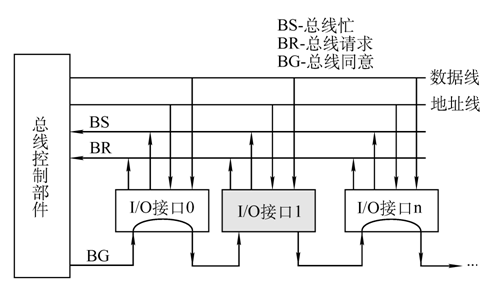
\includegraphics[width=3.12500in,height=1.83333in]{png-jpeg-pics/C709FC82AD5DDD69C9A5E4CD5A47F06F.png}

\textbf{链式查询优先级判别方式:}离总线控制器越近的部件,其优先级越高;离总线控制器越远的部件,其优先级越低。

{\textbf{2. 计数器查询方式}}

计数器定时查询方式采用一个计数器控制总线使用权(计数器在总线控制部件里面)。相对于链式查询方式多了一组设备地址线,少了一根总线同意线。各个设备仍共用一条请求线,计数器查询方式如下图所示。

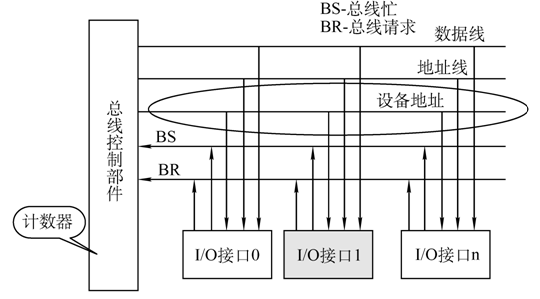
\includegraphics[width=3.33333in,height=1.84375in]{png-jpeg-pics/2677CCDADE787D6529C556368B7549A1.png}

\textbf{计数器查询优先级判别方式:}当总线控制器收到总线请求信号判断总线不忙时,计数器开始计数,计数值通过一组地址线发向各个部件。当地址线上的计数值与请求使用总线设备的地址一致时,该设备获得总线控制权。同时,终止计数器的计数及查询工作。

\textbf{计数器有两种计数方式:}

\textbf{①
计数器每次判优都从``0''开始,}此时一旦设备的优先顺序被固定后,设备的优先级就按0,1,2,,n的顺序降序排列,永远不能改变;

\textbf{②
计数器也可以从上一次的终点开始计数,}即是一种循环方法,此时所有设备使用总线的优先级相等。计数器的初值当然也可以由程序设置,故优先级顺序可以改变。

\textbf{{3. 独立请求方式}}

独立请求方式如下图所示。每一个设备均有一对总线请求信号BRi和总线同意信号BGi。

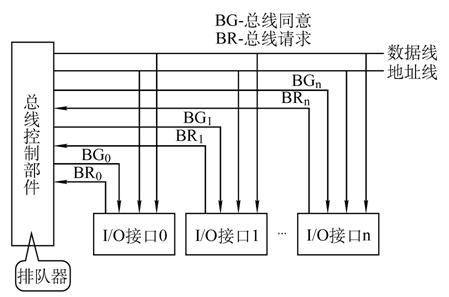
\includegraphics[width=3.33333in,height=2.20833in]{png-jpeg-pics/C58AA5C5E93045826E3C4BA51215C2B3.png}\\
\textbf{独立请求优先级判别方式:}当总线上的部件需要使用总线时,经各自的总线请求线发送总线请求信号,在总线控制器中排队(总线控制部件中有一个排队器)。当总线控制器按一定的优先顺序决定批准某个部件的请求时,则给该部件发送总线响应信号,该部件接到此信号就获得了总线使用权,开始传输数据。
